\section{Anhang}\label{sec:anhang}
\subsection{Bilder Konzeptionierung}\label{subsec:bilder-konzeptionierung}

\begin{figure}[htbp]
    \centering
    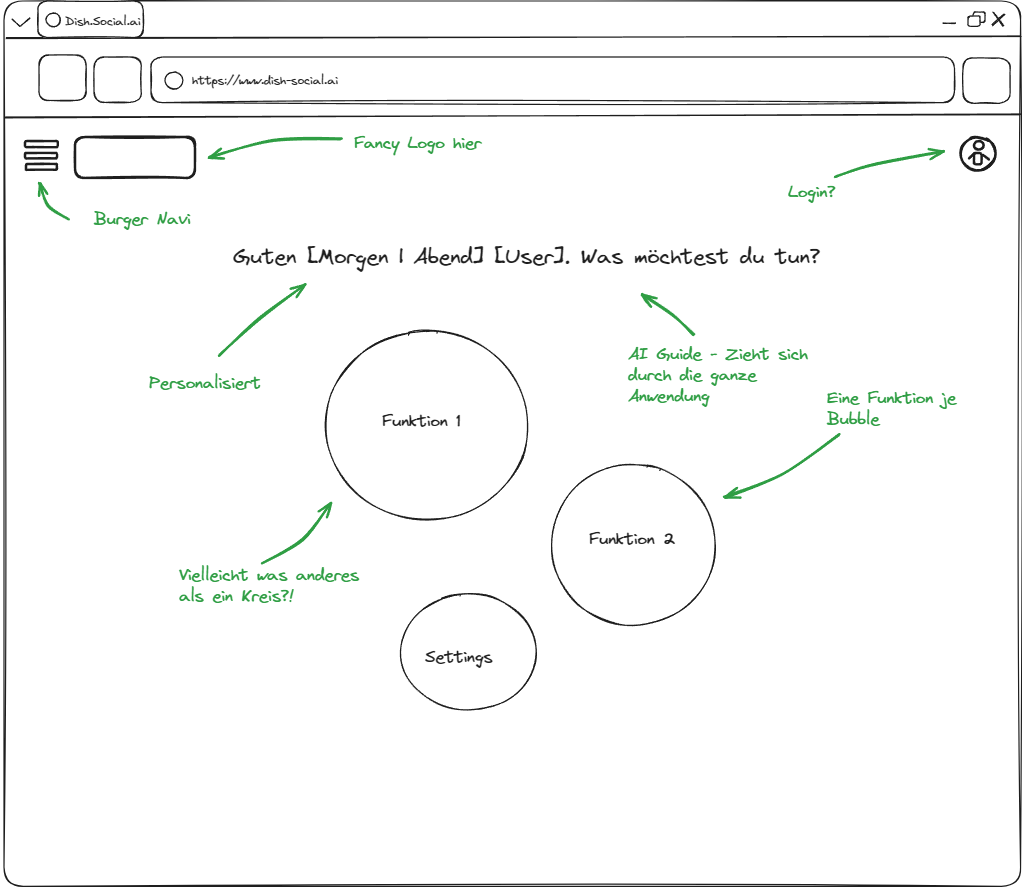
\includegraphics[width=\textwidth]{abbildungen/Konzept/Konzept Landing Page}
    \caption{Figma Design Landing Page}
    \label{fig:landing-page-concept}
\end{figure}
\newpage

\begin{figure}[htbp]
    \centering
    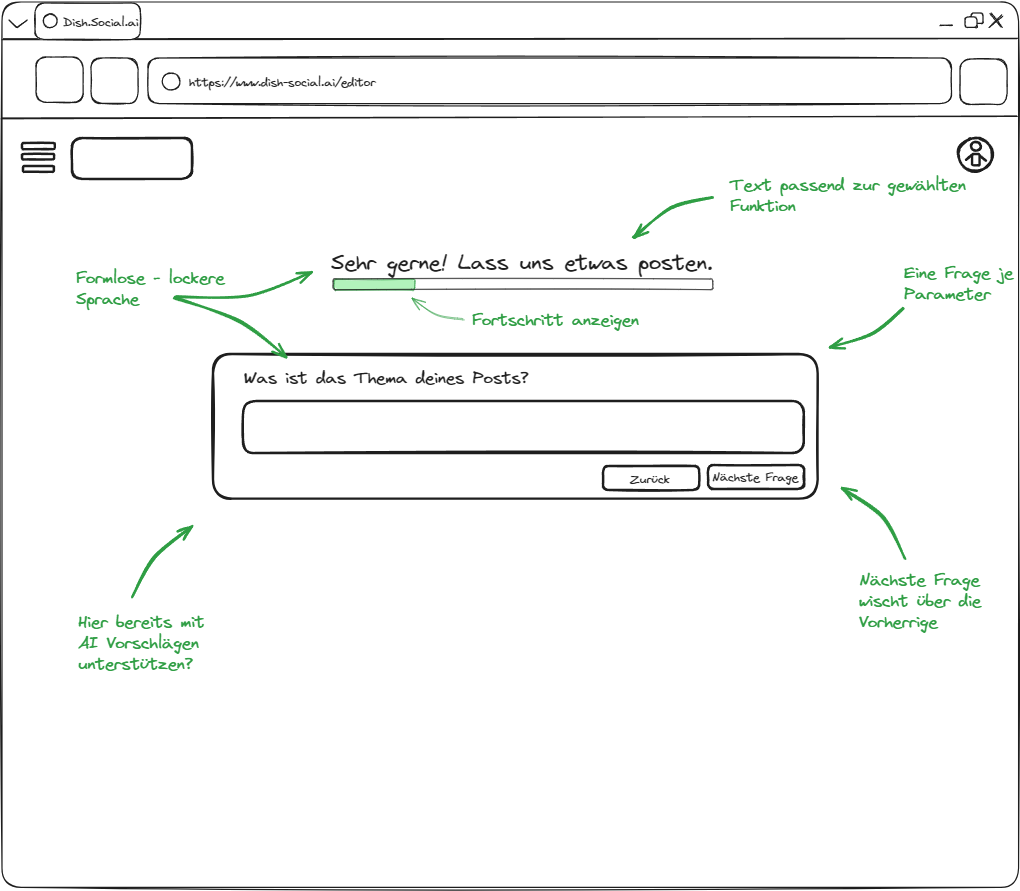
\includegraphics[width=\textwidth]{abbildungen/Konzept/Konzept Dialog}
    \caption{Figma Design Landing Page}
    \label{fig:dialog-concept}
\end{figure}
\newpage

\begin{figure}[htbp]
    \centering
    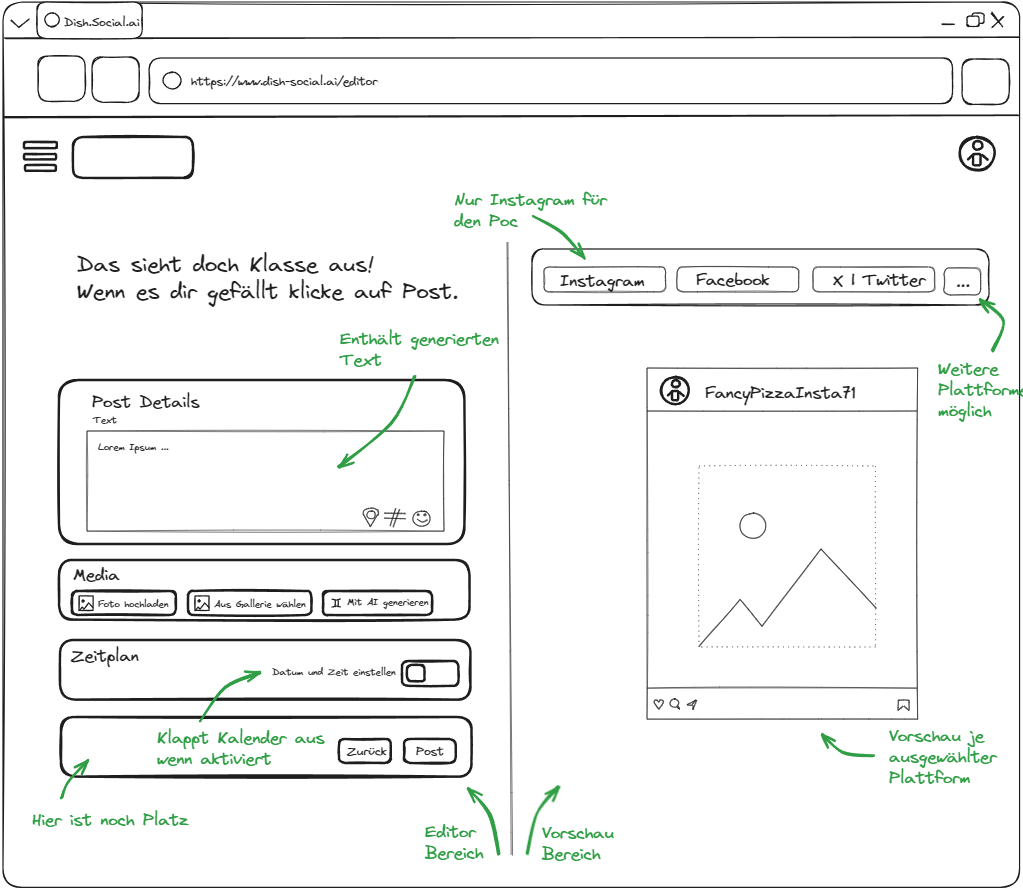
\includegraphics[width=\textwidth]{abbildungen/Konzept/Konzept Editor}
    \caption{Figma Design Landing Page}
    \label{fig:editor-concept}
\end{figure}
\newpage

\begin{figure}[htbp]
    \centering
    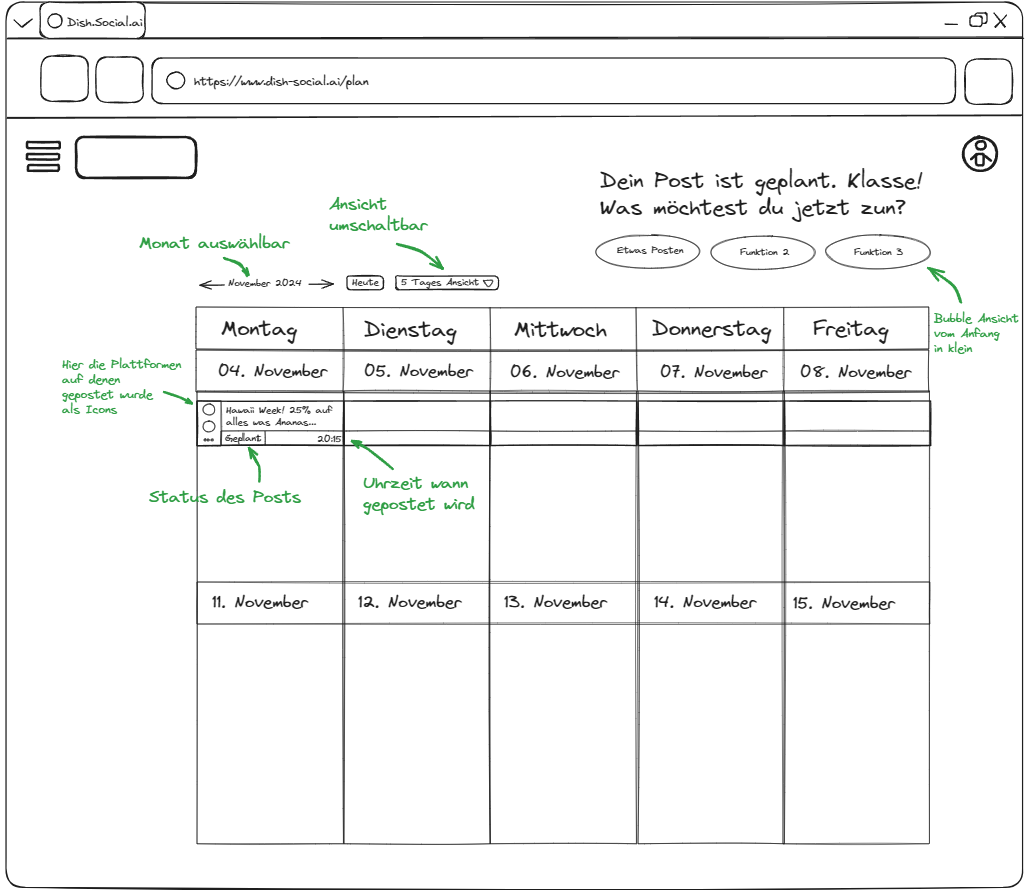
\includegraphics[width=\textwidth]{abbildungen/Konzept/Konzept Kalender}
    \caption{Figma Design Landing Page}
    \label{fig:calendar-concept}
\end{figure}
\newpage

\subsection{Bilder Figma Design}\label{subsec:bilder-figma-design}
\begin{figure}[htbp]
    \centering
    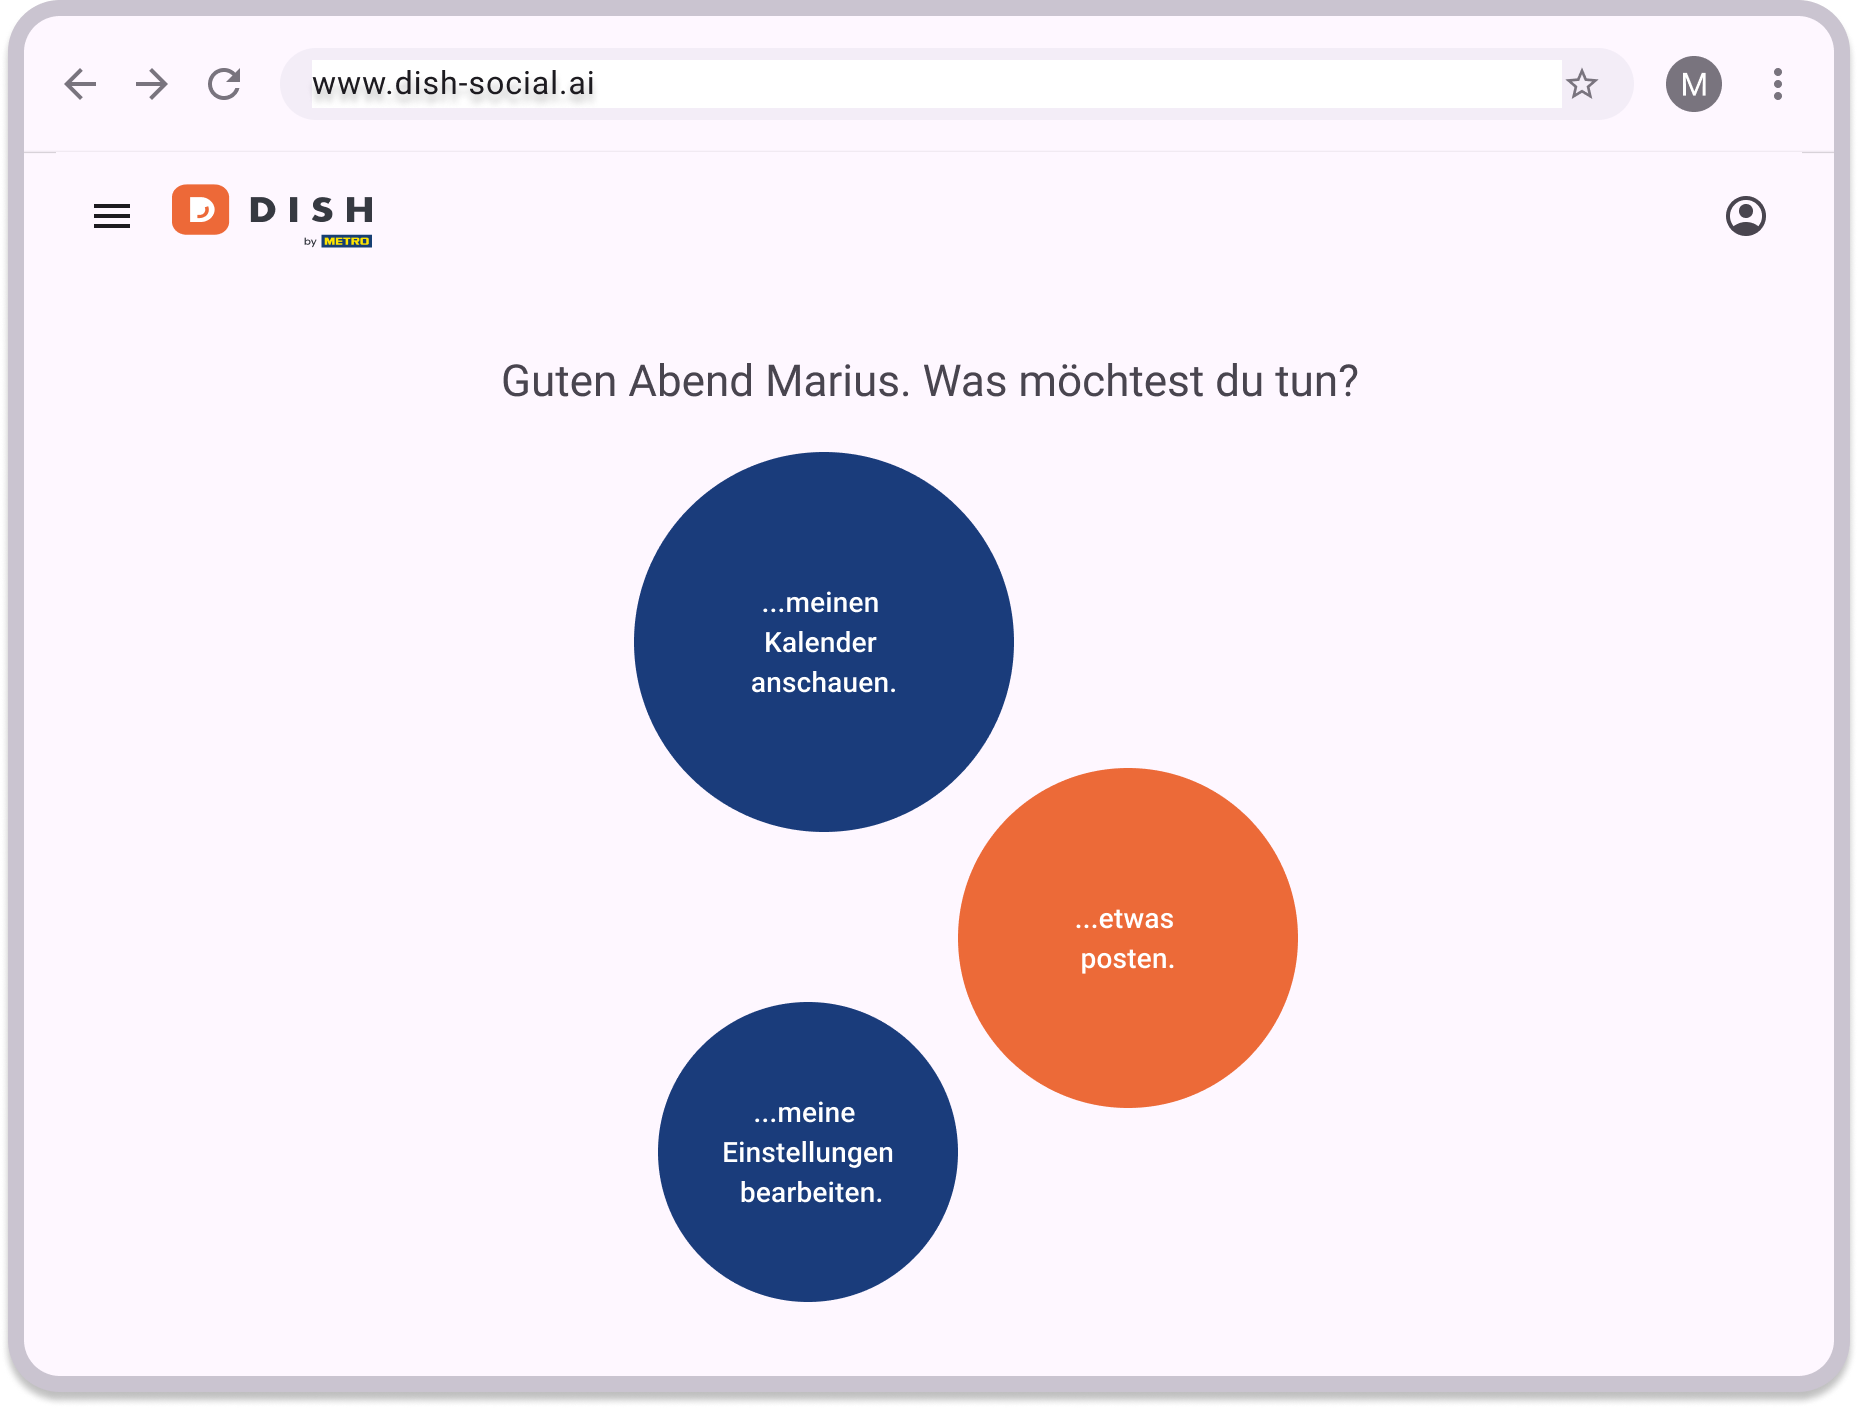
\includegraphics[width=\textwidth]{abbildungen/figma/Landing Page}
    \caption{Figma Design Landing Page}
    \label{fig:landing-page}
\end{figure}
\newpage

\begin{figure}[htbp]
    \centering
    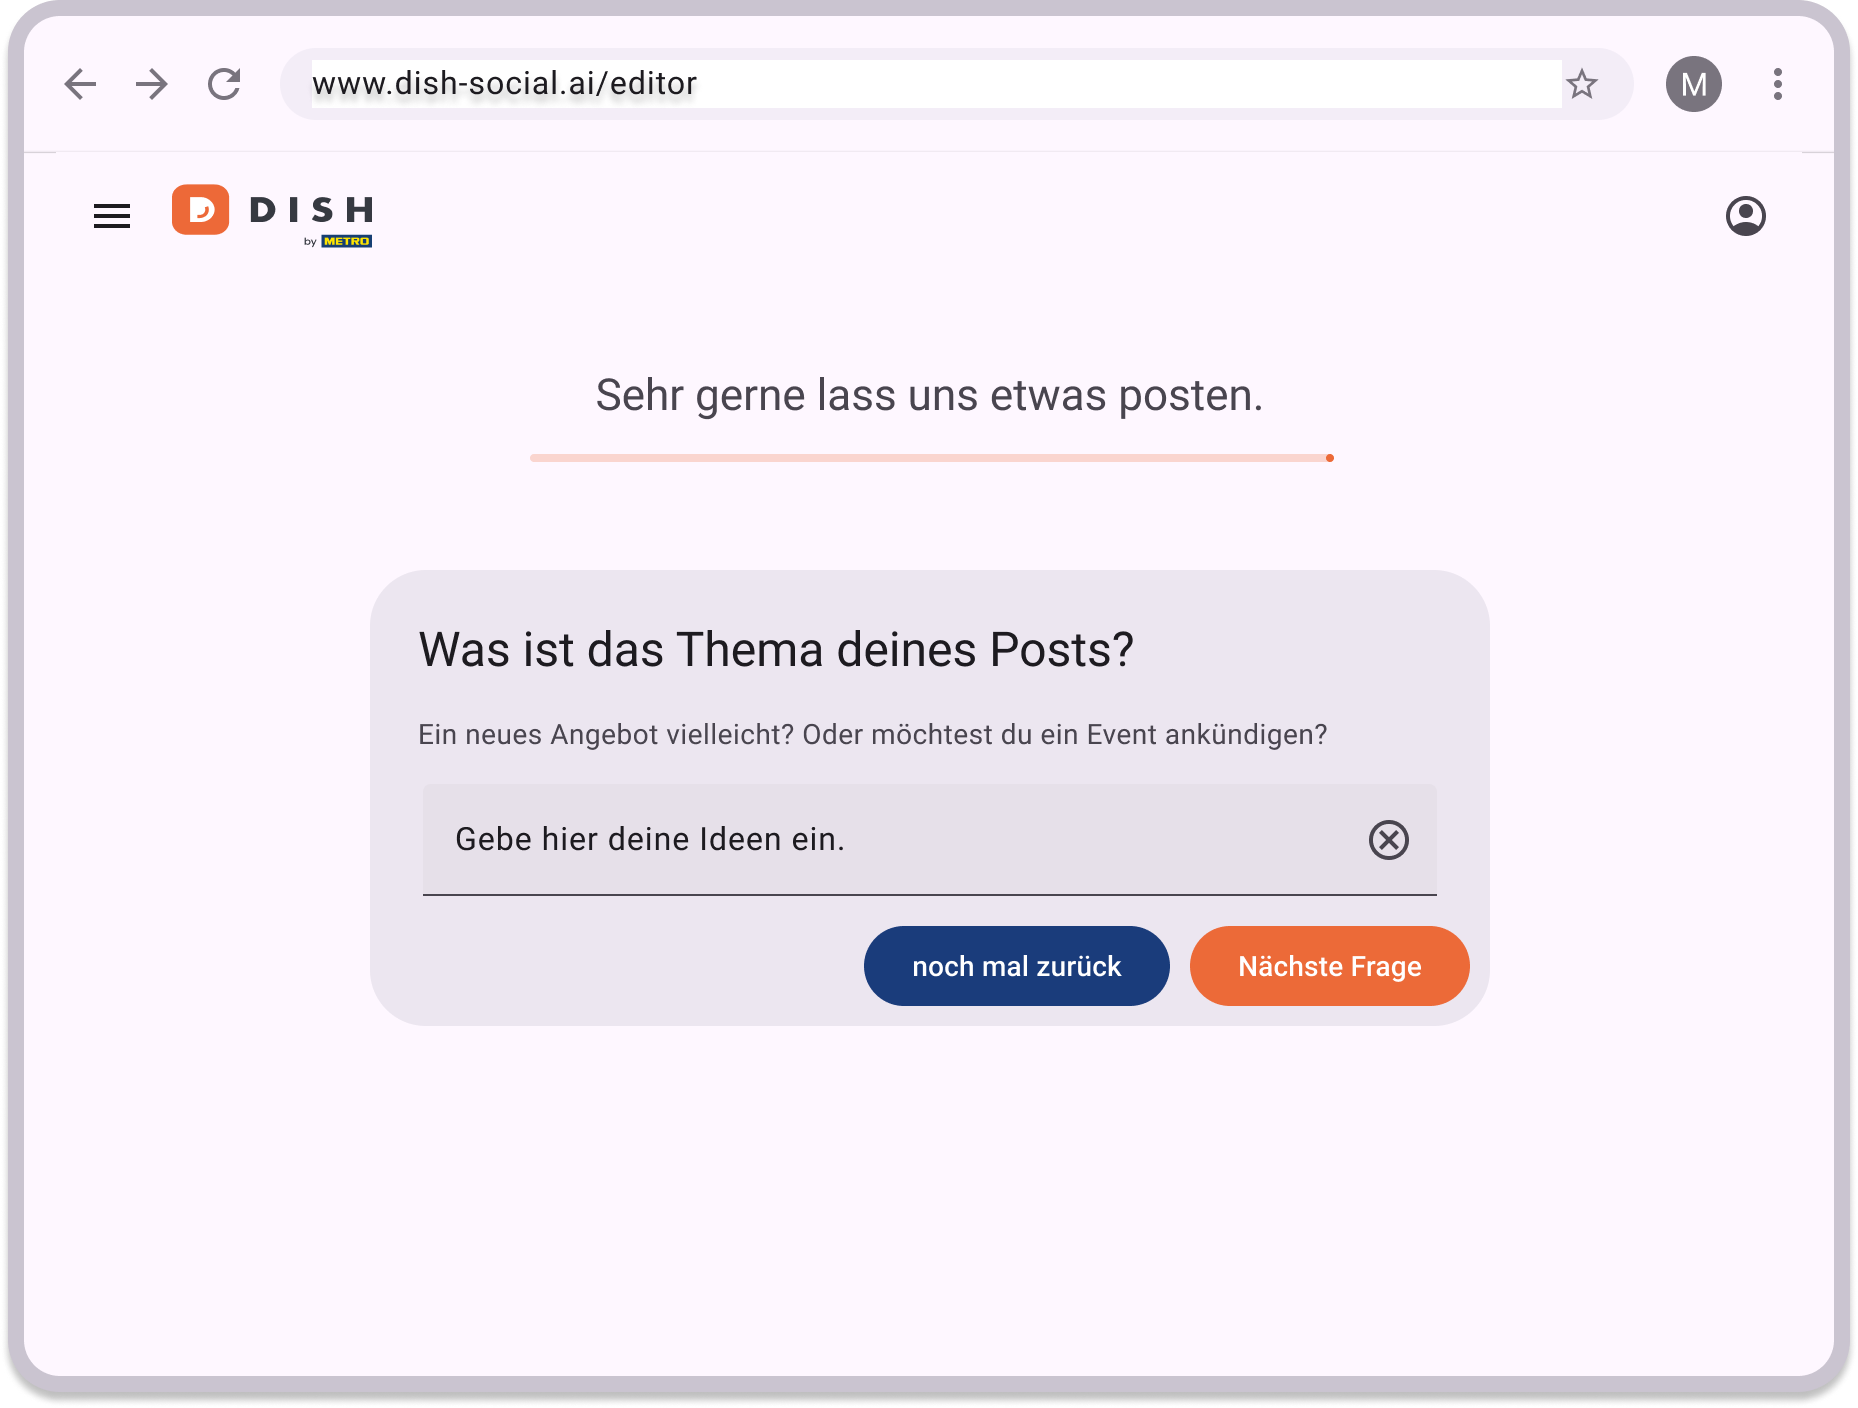
\includegraphics[width=\textwidth]{abbildungen/figma/Dialog}
    \caption{Figma Design Landing Page}
    \label{fig:dialog-page}
\end{figure}
\newpage

\begin{figure}[htbp]
    \centering
    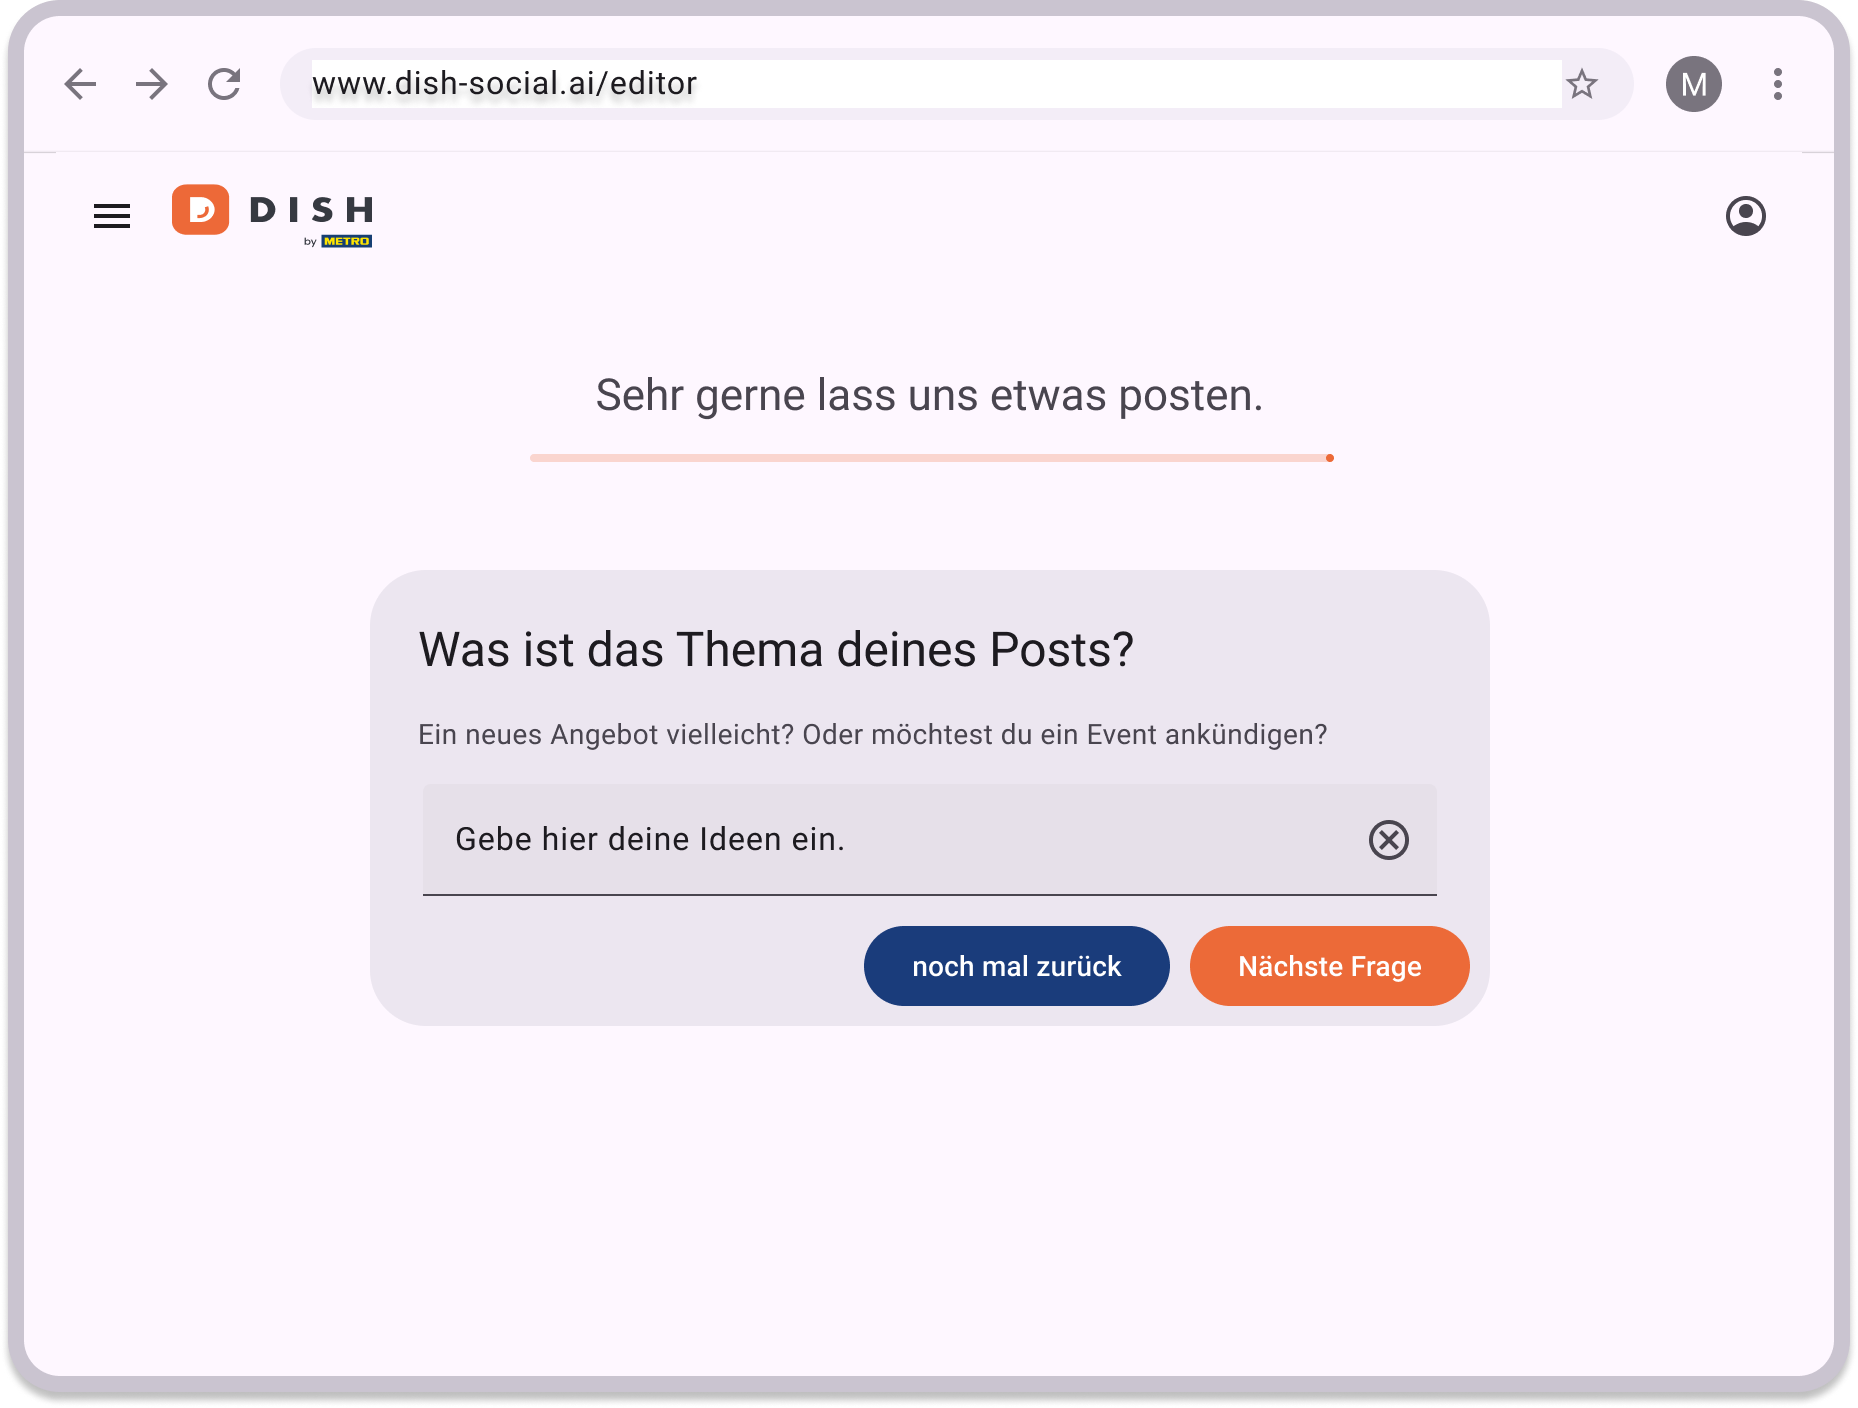
\includegraphics[width=\textwidth]{abbildungen/figma/Editor}
    \caption{Figma Design Landing Page}
    \label{fig:editor-page}
\end{figure}
\newpage

\begin{figure}[htbp]
    \centering
    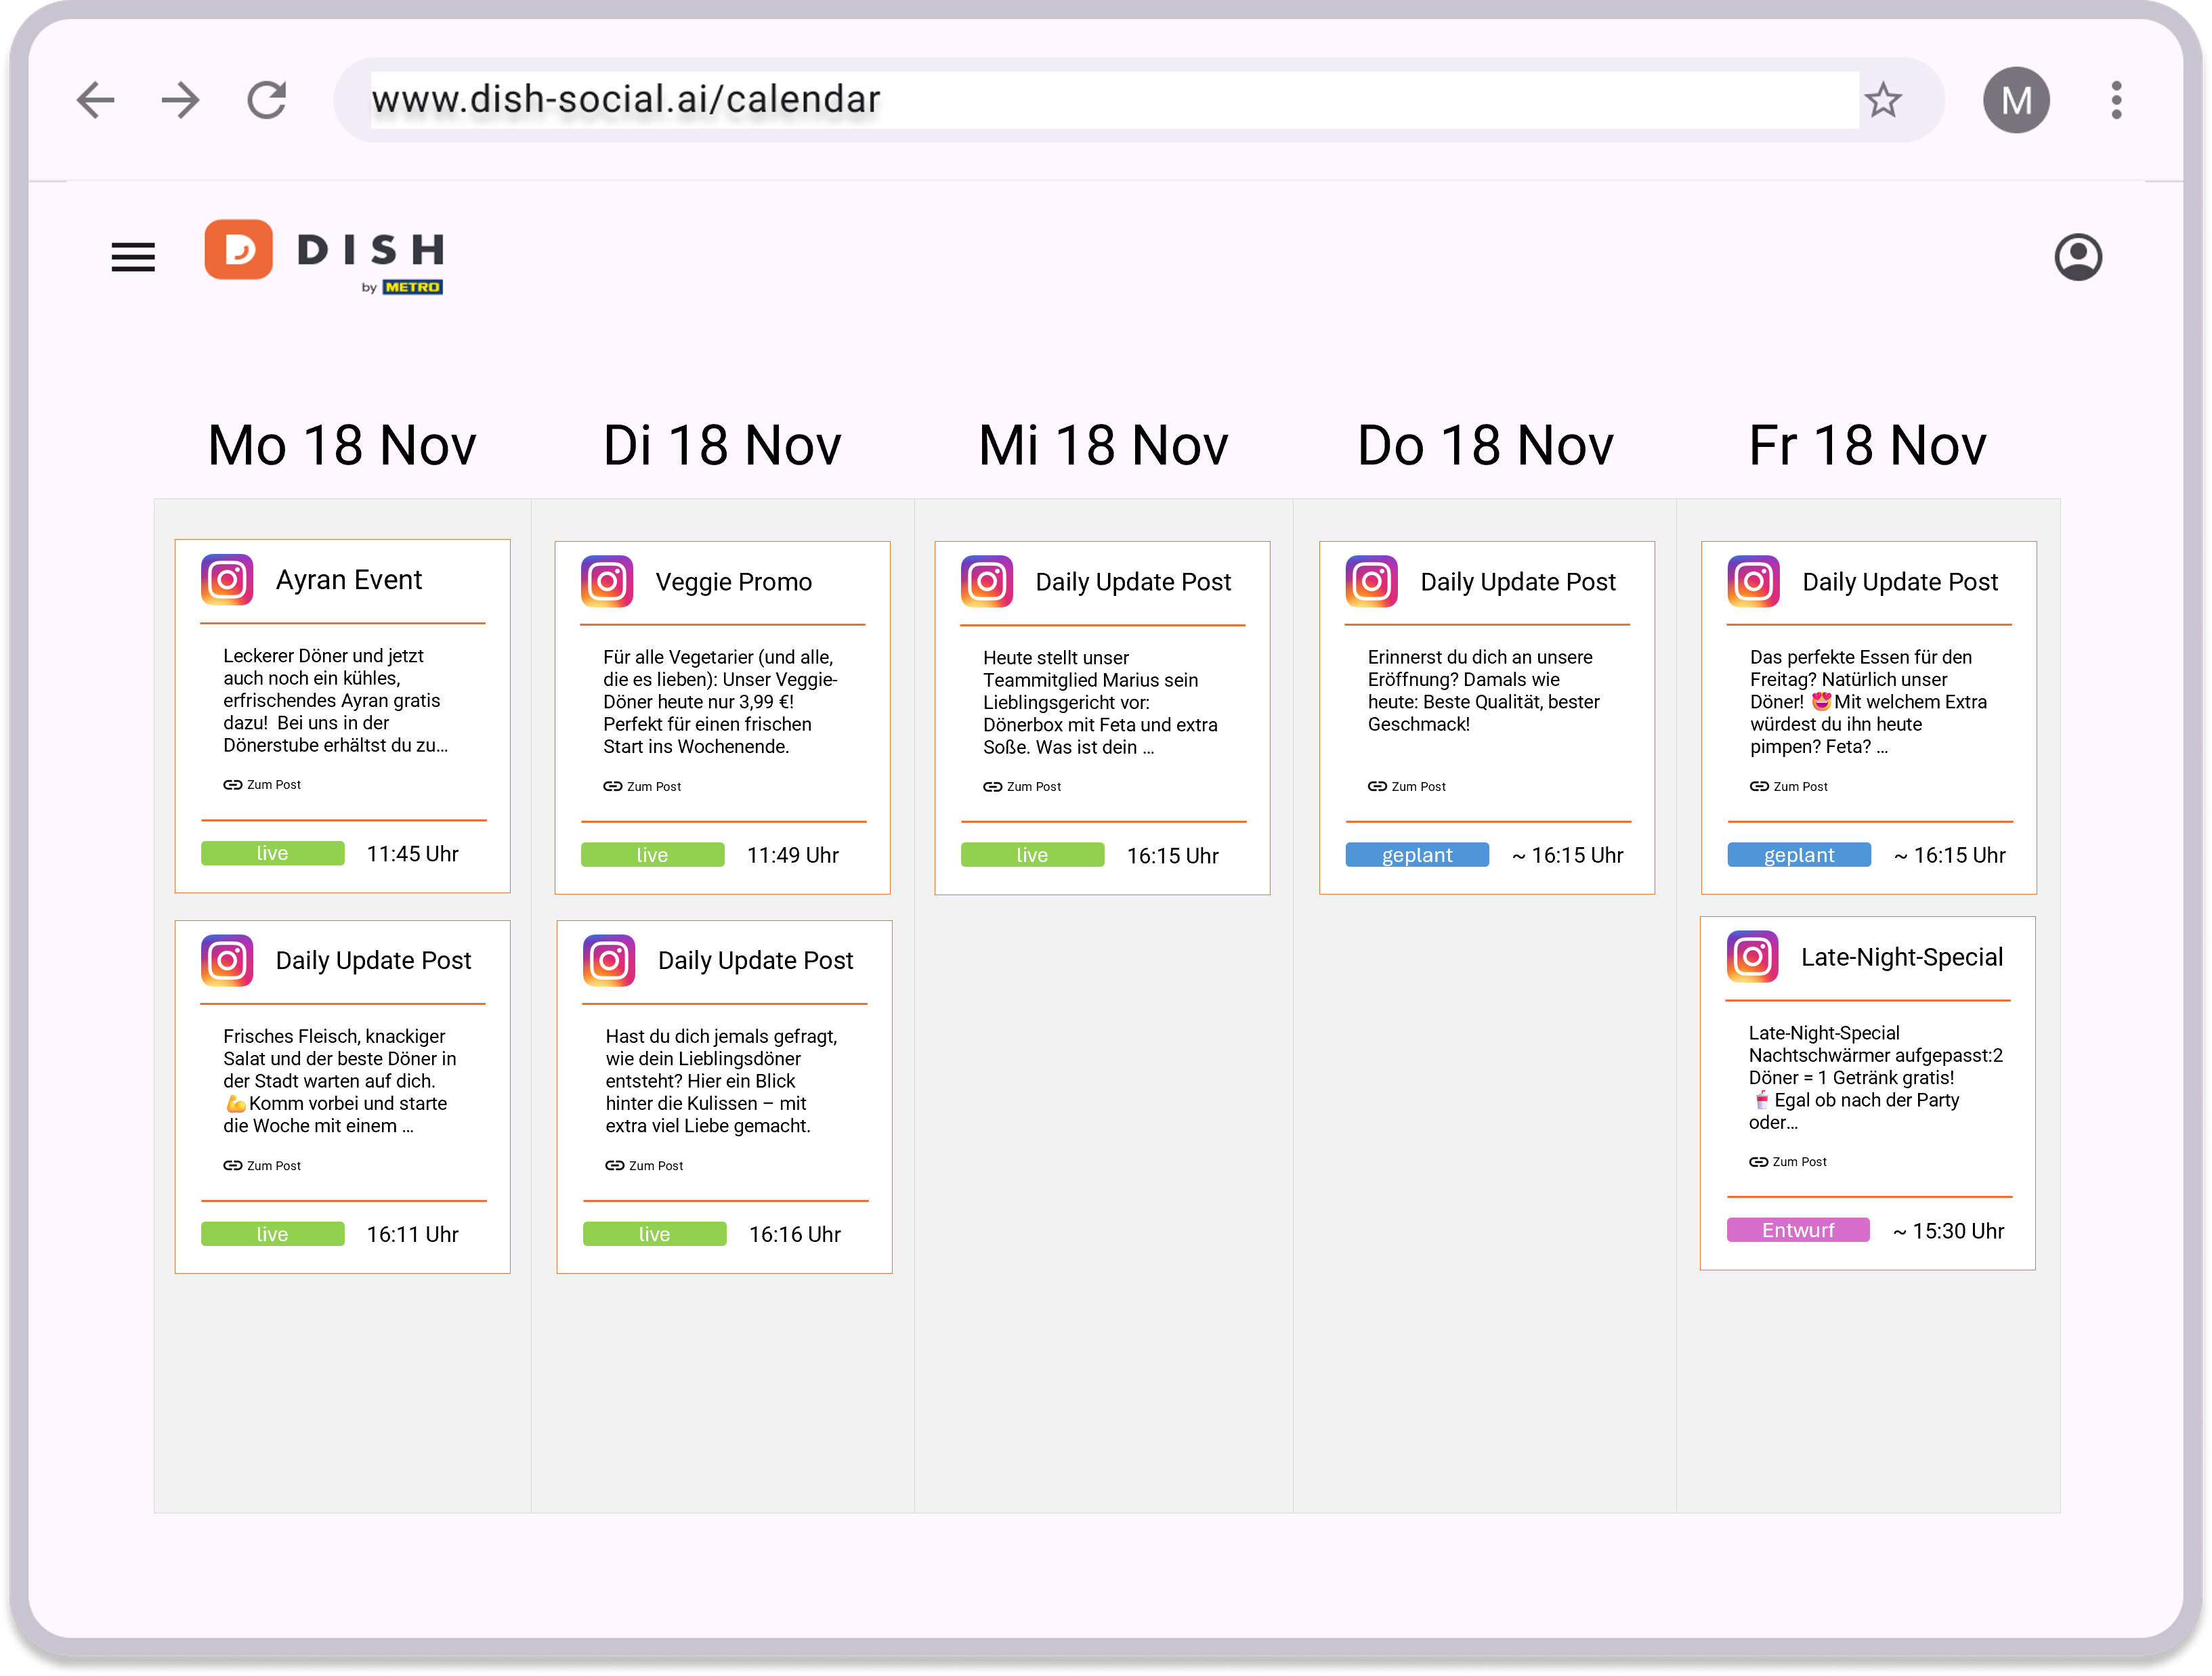
\includegraphics[width=\textwidth]{abbildungen/figma/Kalender}
    \caption{Figma Design Landing Page}
    \label{fig:calendar-page}
\end{figure}